\documentclass[12pt, letterpaper]{article}

\usepackage{tikz}
\usepackage{pgfplots}
\usepackage{amsmath}

\title{Homework 1}
\author{Martin Mueller}
\date{Due: February $8^{th}$, 2019}

\begin{document}
\maketitle

1.

\qquad a) Below is a stem and leaf plot of various distances in miles. The leaves represent the tenths place.
\begin{table}[h!]{ \ \ \ }
	\centering
	\begin{tabular}{r|l}
		\textbf{Stem} & \textbf{Leaf} \\ \hline
        25 & 6 \\
        26 & 4 \\
        27 & \\
        28 & 3, 8 \\
        29 & 4, 8 \\
        30 & 4, 6, 6, 9 \\
        31 & 0, 4, 5, 6, 6, 8 \\
        32 & 2, 2, 4, 5, 5 \\
        33 & 0, 2, 5, 6 \\
        34 & 1, 2, 3, 3, 4, 5, 5, 6, 8, 8 \\
        35 & 2, 2, 2, 2, 4 \\
        36 & 3 \\
        37 & 1, 6 \\
        38 & \\
        39 & 6 \\
        40 & \\
        41 & \\
        42 & 0 \\
	\end{tabular}
\end{table}

\pagebreak

\qquad b) The histogram below lists the number of data points in the stem and leaf plot on the previous page. Each bar represents the number of data points between the listed number and the number after it, (e.g. 24 represents the number of data points as listed in the stem and leaf plot in the rows labeled 24 and 25).
\begin{center}
	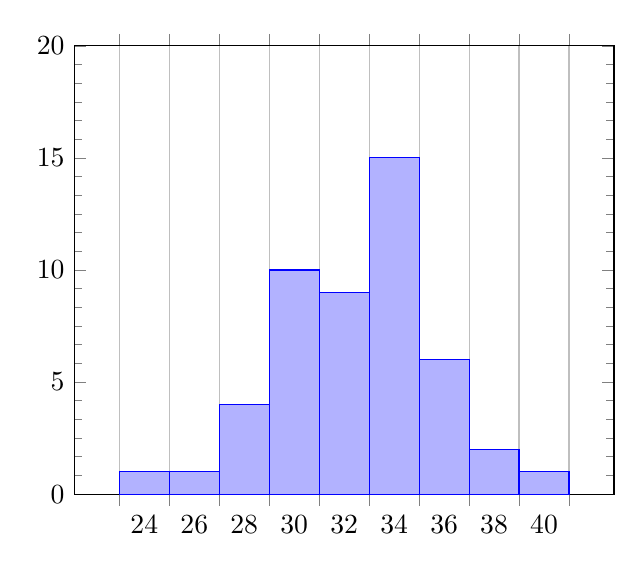
\begin{tikzpicture}
		\begin{axis}[
			ybar interval,
			ymax=20,ymin=0,
			minor y tick num = 5
			]
			\addplot coordinates { (24, 1) (26, 1) (28, 4) (30, 10) (32, 9) (34, 15) (36, 6) (38, 2) (40, 1) (42, 1) };
		\end{axis}
	\end{tikzpicture}
\end{center}

\qquad c) Below lists the mean and 20 percent trimmed mean for the data points listed in $1a$. The mean was calculated by simply adding up each data point, then dividing by the number of data points, in this case 45. The 20 percent trimmed mean was calculated by removing 20 percent of the data points from each end, in this case 11 data points from each end.

$$\text{mean} = \frac{\sum\limits_{i=1}^{45} n_{i}}{45} = \boxed{33.0}$$

$$\text{20\% trimmed mean} = \frac{\sum\limits_{i=12}^{34} n_{i}}{23} = \boxed{33.2}$$

\pagebreak

2.

\qquad a) Below is a stem and leaf plot of various times in minutes. The leaves represent the tenths place.
\begin{table}[h!]{ \ \ \ }
	\centering
	\begin{tabular}{r|l}
		\textbf{Stem} & \textbf{Leaf} \\ \hline
        12 & 4 \\
        13 & 9\\
        14 & 3, 8\\
        15 & 4, 6, 8\\
        16 & 4, 6, 6\\
        17 & 0, 4, 5, 6, 6, 8\\
        18 & 0, 2, 2, 4, 5, 5, 7\\
        19 & 0, 2, 4, 5, 6, 6, 7\\
        20 & 1, 2, 3, 3, 4, 5, 5, 6, 8, 8\\
        21 & 2, 2, 2, 2, 4\\
        22 & 3\\
        23 & 1, 1, 6\\
        24 & \\
        25 & 6\\
	\end{tabular}
\end{table}

\qquad b) The histogram below lists the number of data points in the stem and leaf plot above. Each bar represents the number of data points between the listed number and the number after it, (e.g. 12 represents the number of data points as listed in the stem and leaf plot in the rows labeled 12 and 13).
\begin{center}
	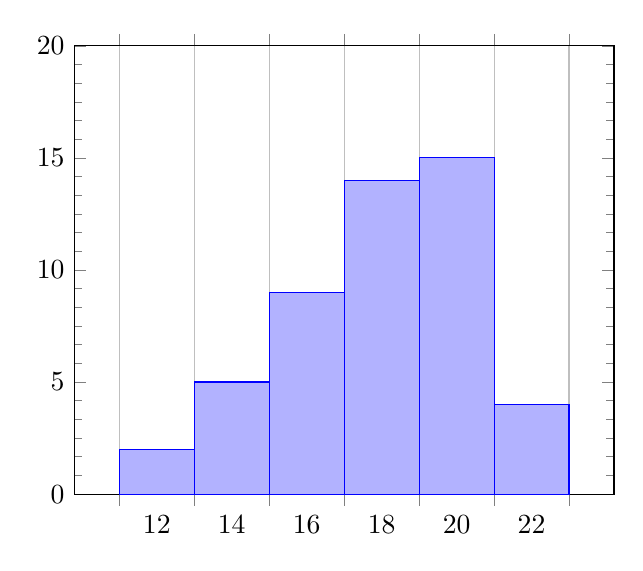
\begin{tikzpicture}
		\begin{axis}[
			ybar interval,
			ymax=20,ymin=0,
			minor y tick num = 5
			]
			\addplot coordinates { (12, 2) (14, 5) (16, 9) (18, 14) (20, 15) (22, 4) (24, 1) };
		\end{axis}
	\end{tikzpicture}
\end{center}

\pagebreak

\qquad c) Below lists the mean and 8 percent trimmed mean for the data points listed in $2a$. The mean was calculated by simply adding up each data point, then dividing by the number of data points, in this case 50. The 8 percent trimmed mean was calculated by removing 8 percent of the data points from each end, in this case 4 data points from each end.

$$\text{mean} = \frac{\sum\limits_{i=1}^{50} n_{i}}{50} = \boxed{19.0}$$

$$\text{8\% trimmed mean} = \frac{\sum\limits_{i=5}^{46} n_{i}}{42} = \boxed{18.9}$$

\end{document}